\chapter{Theorie}\label{ch:data}

\section{Grafische Benutzeroberfläche}
Benutzerschnittstelle bezeichnet alle Komponenten eines interaktiven Systems, die dem Benutzer Interaktionsmöglichkeiten mit selbigem System bieten um ein verfolgtes Ziel zu erreichen.
Die grafische Benutzeroberfläche (GUI) bezeichnet hierbei den sichtbaren Anteil des Systems und damit nur einen Teil der gesamten Benutzerschnittstelle, zu der auch nicht sichtbare Teile wie z.B. die Funktionslogik beinhaltet sind.\cite{Sarodnick.2016}
Heutzutage sind die meisten Benutzeroberflächen auch grafische Benutzeroberflächen, mit denen in den häufigsten Fällen die Interaktion  über direkte Manipulation stattfindet.\cite{Nielsen.1995?}

\section{Definition Ergonomie}
Unter Ergonomie versteht man im Allgemeinen die "Lehre von der menschlichen Arbeit und die Erkenntnis ihrer Gesetzmäßigkeiten"\cite{https:www.facebook.comArbeitsplatzergonomie.2014}.
Hierbei ist es wichtig zu verstehen, dass dabei der Fokus nicht ausschließlich auf einer technischen Komponente liegt, sondern das Zusammenspiel von Mensch, der zugeteilten Aufgabe und den verfügbaren Werkzeugen betrachtet wird\cite{Sarodnick.2016}.
Im Bezug auf Software bedeutet Ergonomie also konkret diese gut handhabbar und benutzerorientiert zu gestalten.

\section{Definition Usability}
Mit immer höherer Komplexität von Systemen und Anwendungen kam der Begriff und das Verlangen nach  "Benutzerfreundlichkeit"\ auf.
Dieser Begriff suggeriert das lediglich die einfache Benutzung eines Systems ausschlaggebend ist, vernachlässigt hierbei jedoch die Notwendigkeit den Nutzer beim Erreichen seiner Ziele passend zu unterstützen.
Dies ist auch der Grund dafür das bald, statt auf "Benutzerfreundlichkeit"\ auf "Gebrauchstauglichkeit" (engl. Usability) geachtet wurde.
Im Gegensatz zur Ergonomie handelt es sich bei Usability nicht um eine eigenständige wissenschaftliche Disziplin, sondern um eine qualitative Anforderung an ein System\cite{Sarodnick.2016}.
Konkret spricht man bei einer Software-Anwendung von einer hohen Usability, wenn sie von der für sie bestimmten Zielgruppe effizient verwendet werden kann, also das verfolgte Ziel zufriedenstellend erreicht wird\cite{Richter.2016}.
Hierfür ist es entscheidend sich bewusst zu machen das ein technisches System oder Software immer Teil eines großen Handlungsablaufes ist und dazu dient Schritte dieses Handlungsablaufes zu erledigen.
Deshalb muss das System den Anforderungen dieses Ablaufes entsprechen und darf während der Entwicklung nicht getrennt davon betrachtet werden\cite{Sarodnick.2016}.

\section{Definition User Experience}
Entgegen einer häufigen Annahme bezeichnen Usability und User Experience (UX) nicht das Gleiche.
Tatsächlich ist Usability lediglich ein Teil der gesamten User Experience eines Systems\cite{Knight.2019c}.
UX bezieht sich nicht nur auf die reine Nutzungszeit eines Systems, sondern berücksichtigt auch den Zeitraum davor und danach, bezeichnet als Antizipierte Nutzung und Verarbeitung der Nutzungssituation.
Usability ist hierbei, wie in \cref{fig:UX} zu sehen,  als wichtiger Faktor der User Experience in der aktiven Nutzungsphase zu betrachten, jedoch nicht mit dem Begriff gleichzusetzen \cite{Sarodnick.2016}.
Durch die zusätzliche Betrachtung der Effekte auf den Nutzer vor und nach der Nutzung, wie beispielsweise Erwartungen an das Produkt und Akzeptanz des selbigen, entstehen hier auch Verbindungen zur Gestaltung der Benutzerschnittstelle und dem Produkt-Design\cite{Richter.2016}.
Zusammenfassend lässt ich festhalten das Usability zwar die funktionsbezogene Betrachtungsweise abdeckt, die User Experience als ganzes jedoch auch emotionale Faktoren bezüglich Design und Ästhetik berücksichtigt um das Nutzungsvergnügen möglichst hoch zu halten.
Zusätzlich ist eine gute User Experience notwendig wenn ein Produkt auf dem Markt bestehen will.
Sobald es mehr als ein Produkt zur Lösung der gleichen Aufgabenstellung gibt, wird das mit der besseren User Experience Verwendung finden\cite{Knight.2019c}.

\begin{figure} [!h]
\begin{center}
  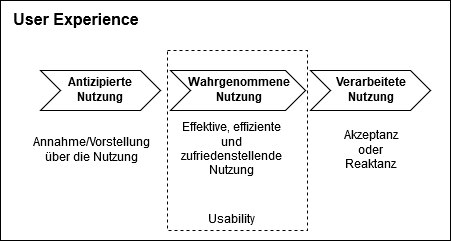
\includegraphics[scale=0.7]{figures/UX.png}
  \caption{Zusammenhang Usability und User Experience (nach \cite{Sarodnick.2016})}
  \label{fig:UX}
\end{center}
\end{figure}

\section{Human - Centered - Design - Process}
TODO

\begin{figure} [!h]
\begin{center}
  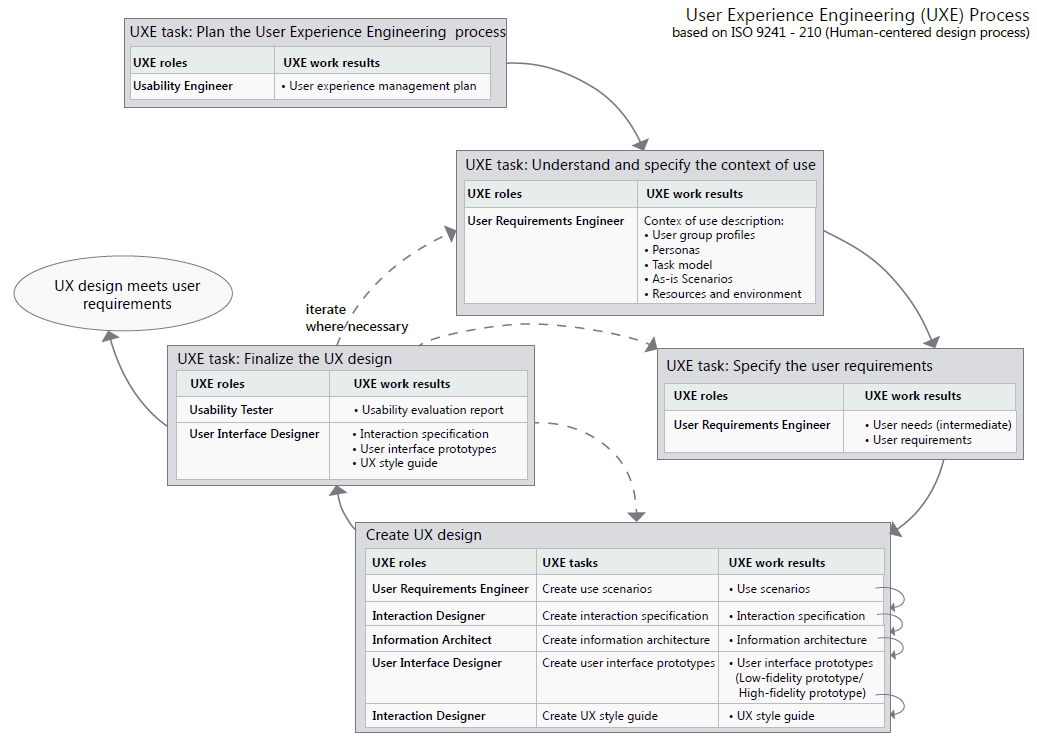
\includegraphics[width=\textwidth]{figures/HCD.png}
  \caption{Human - Centered - Design - Process bei Elektrobit}
  \label{fig:HCD}
\end{center}
\end{figure}

\section{Gestaltprinzipien der Usability}
TODO Notizen fertig machen
TODO Ausformulieren

\cite{Norman.2016} Für Einleitung etwas suchen

\subsection{Konsistenz}
Systeme sind benutzbarer wenn gleiche Funktionen auch die gleiche Darstellung haben.
Ermöglicht es bereits Gelerntes im neuen Kontext anzuwenden, dadurch schnell neue Fähigkeiten zu lernen, und den Fokus auf relevante neue Aspekte zu legen.

Ästhetische Konsistenz bezieht sich auf den Stil und Aussehen, z.B eines Logos. 

Funktionale Konsistenz bezieht sich auf die Konsistenz von Bedeutung und Aktion, z.B Ampel zeigt orange bevor sie rot wird. Erhöht die Usability und Lernfähigkeit, durch Übertragung bereits erlangten Wissens in die neue Umgebung. z.B Playbutton von Kassettenrekorder zu MP3-Player.

Interne Konsistenz bezieht sich auf Konsistenz mit anderen Elementen im System. Erzeugt Vertrauensgefühl bei den Nutzern, vermittelt durchdachtes Design, kein einfaches zusammenstöpseln von Komponenten. Innerhalb einer logischen Gruppen sollten Elemente ästhetisch und funktional Konsistent sein.

Ästhetische und funktionale Konsistenz sollten in allen Designbereichen berücksichtigt werden.
Ästhetische zur Einführung einmaliger Identitäten um Wiedererkennung zu gewährleisten.
Funktionale für gute Usability.
Systeme sollten immer eine interne Konsistenz aufweisen, wenn es bereits Designstandards gibt sollten diese analysiert werden.
\cite{Lidwell.2010}

\subsection{Sichtbarkeit}
Systeme sind benutzbarer wenn der aktuelle Status eindeutig zu erkennen ist, die möglichen Aktionen die ausgeführt werden können, und die Auswirkungen der ausgeführten Aktionen.
Prinzip baut auf der Erkenntnis auf das Menschen Lösungswege erkennen können wenn sie aus einer Anzahl von Optionen auswählen können, als wenn sie sich an einzelne Schritte aus dem Stegreif erinnern müssen.
Für komplexe Systeme ist dieses Prinzip daher das wichtigste für eine gute Usability.
häufig wird versucht alle möglichen Optionen die ein System bietet sichtbar zu machen, was dazu führt das die relevanten Optionen schwerer zu erreichen sind weil eine Informationsüberladung beim Nutzer stattfindet.
Als Lösung bietet sich eine Hierarchische Organisation oder Kontextsensitivität an.
Hierarchische platziert Funktionen und Informationen in logische Kategorien und versteckt sie mit einer übergeordneten Kontrolle, wie zum Beispiel einem Softwaremenü.
Kontextsensitive zeigt oder versteckt Aktionsmöglichkeiten und Informationen abhängig vom aktuellen Status des Systems.
\cite{Lidwell.2010}

\subsection{Affordanz}
Visuelle Eigenschaft eines Elementes das dem Nutzer vermittelt wie mit ihm interagiert werden kann. Im digitalen Umfeld z.B. ein Button.
Ästhetische Eigenschaften eines Buttons müssen visuell vermitteln das er angeklickt werden kann.
Kann visuell gelöst werden indem der Button wie ein Button in der echten Welt aussieht, also ein dreidimensionales Aussehen gewählt wird.
Oder indem der Button komplett anders als der Rest des Interfaces gestaltet wird damit der User versteht das hier eine Interaktion stattfinden kann.\cite{Knight.2019c}

\subsection{Rückmeldung}
Eine Rückmeldung nach der Interaktion eines Nutzers, verdeutlicht diesem das die von ihm beabsichtigte Aktion ausgeführt wurde, ob sie erfolgreich war oder nicht ändert nichts an der Tatsache das eine Rückmeldung nötig ist.
Kommt gar keine Rückmeldung vom System kann der Nutzer nicht zuordnen ob überhaupt eine Aktion ausgeführt wurde. Durch fehlende Rückmeldungen kommt Misstrauen beim Nutzer auf, weil ihm nicht vermittelt wird ob auf seine Aktionen auch eine Reaktion des Systems erfolgt.\cite{Knight.2019c}

\subsection{Mapping}
Wenn der Effekt den eine Nutzerinteraktion nach sich zieht, den Erwartungen des Nutzers entspricht, handelt es sich um gutes Mapping. Beispiel elektronisches Fensterheber, Hebel nach oben hebt das Fenster, Hebel nach unten senkt es.

Gutes Mapping ist zum Großteil eine Funktion der Ähnlichkeit eines Layouts, dessen Verhaltens, oder dessen Bedeutung.
Layout Herdplattenregler entspricht der Anordnung der Platten -> Layout
Bewegung Lenkrad -> Verhalten
Notfallknopf in der Farbe rot -> Bedeutung
In jedem dieser Fälle macht die Ähnlichkeit es möglich den Effekt der Handlung vorherzusehen, vereinfacht also die Bedienung.

Aktionsmöglichkeiten müssen so platziert werden das ihre Position und ihr Verhaltend dem Layout und dem Verhalten den Anwendung angepasst sind. Simple Beziehungen zwischen Eingabe und Aktion funktionieren am besten.
Die gleiche Aktion für verschiedene Funktionen zu benutzen sollte vermieden werden.
\cite{Lidwell.2010}
\subsection{Einschränkungen}
Einschränkung der Aktionen die ein Systems ausführen kann, z.B. ausgrauen von Buttons die nicht funktionstüchtig sind.
Richtige Anwendung von Einschränkungen macht ein Design einfacher nutzbar und reduziert deutlich die Wahrscheinlichkeit von Fehlschlägen während der Systeminteraktion.
Zwei Typen von Einschränkungen: Physische und Psychologische \cite{Lidwell.2010}

Mehr bei \cite{Norman.2016}
\subsection{Vorteile für den Nutzer}
Durch die Nutzung bekannter Interfacestrukturen und Funktionalitäten, muss der Nutzer seine Energie nicht darauf verschwenden darüber nachzudenken wie mit den Bestandteilen des Interfaces interagiert werden kann, oder was deren Funktion sein könnte.
\cite{Knight.2019c}

\section{EB Guide Studio}
Wie bereits in Abschnitt 1.2 erwähnt dient EB GUIDE der Entwicklung multimodalder HMIs.
Um nicht nur das Design sondern auch das Verhalten von User Interfaces bestimmen zu können und eine Auslieferung auf das Zielsystem zu ermöglichen besteht die Produktlinie EB GUIDE aus den verschiedenen, in \cref{fig:guide_puzzle} zu sehenden, Komponenten.
Hierbei wird zwischen Komponenten für das Graphical User Interface (GUI) und Komponenten für die Sprachsteuerung unterschieden.
Da die Sprachkomponenten jedoch für diese Arbeit nicht weiter relevant sind werden diese in den folgenden Kapiteln auch nicht genauer erläutert.
Innerhalb des GUI Bereiches bildet EB GUIDE Studio das tatsächliche Modellierungstool mit dem das Verhalten und Aussehen der Benutzeroberfläche definiert wird.
Für das entwickelte Modell stellt das EB GUIDE Target Framework auf dem Zielsystem die Laufzeitumgebung bereit.\cite{.c} 

\begin{figure} [!h]
\begin{center}
  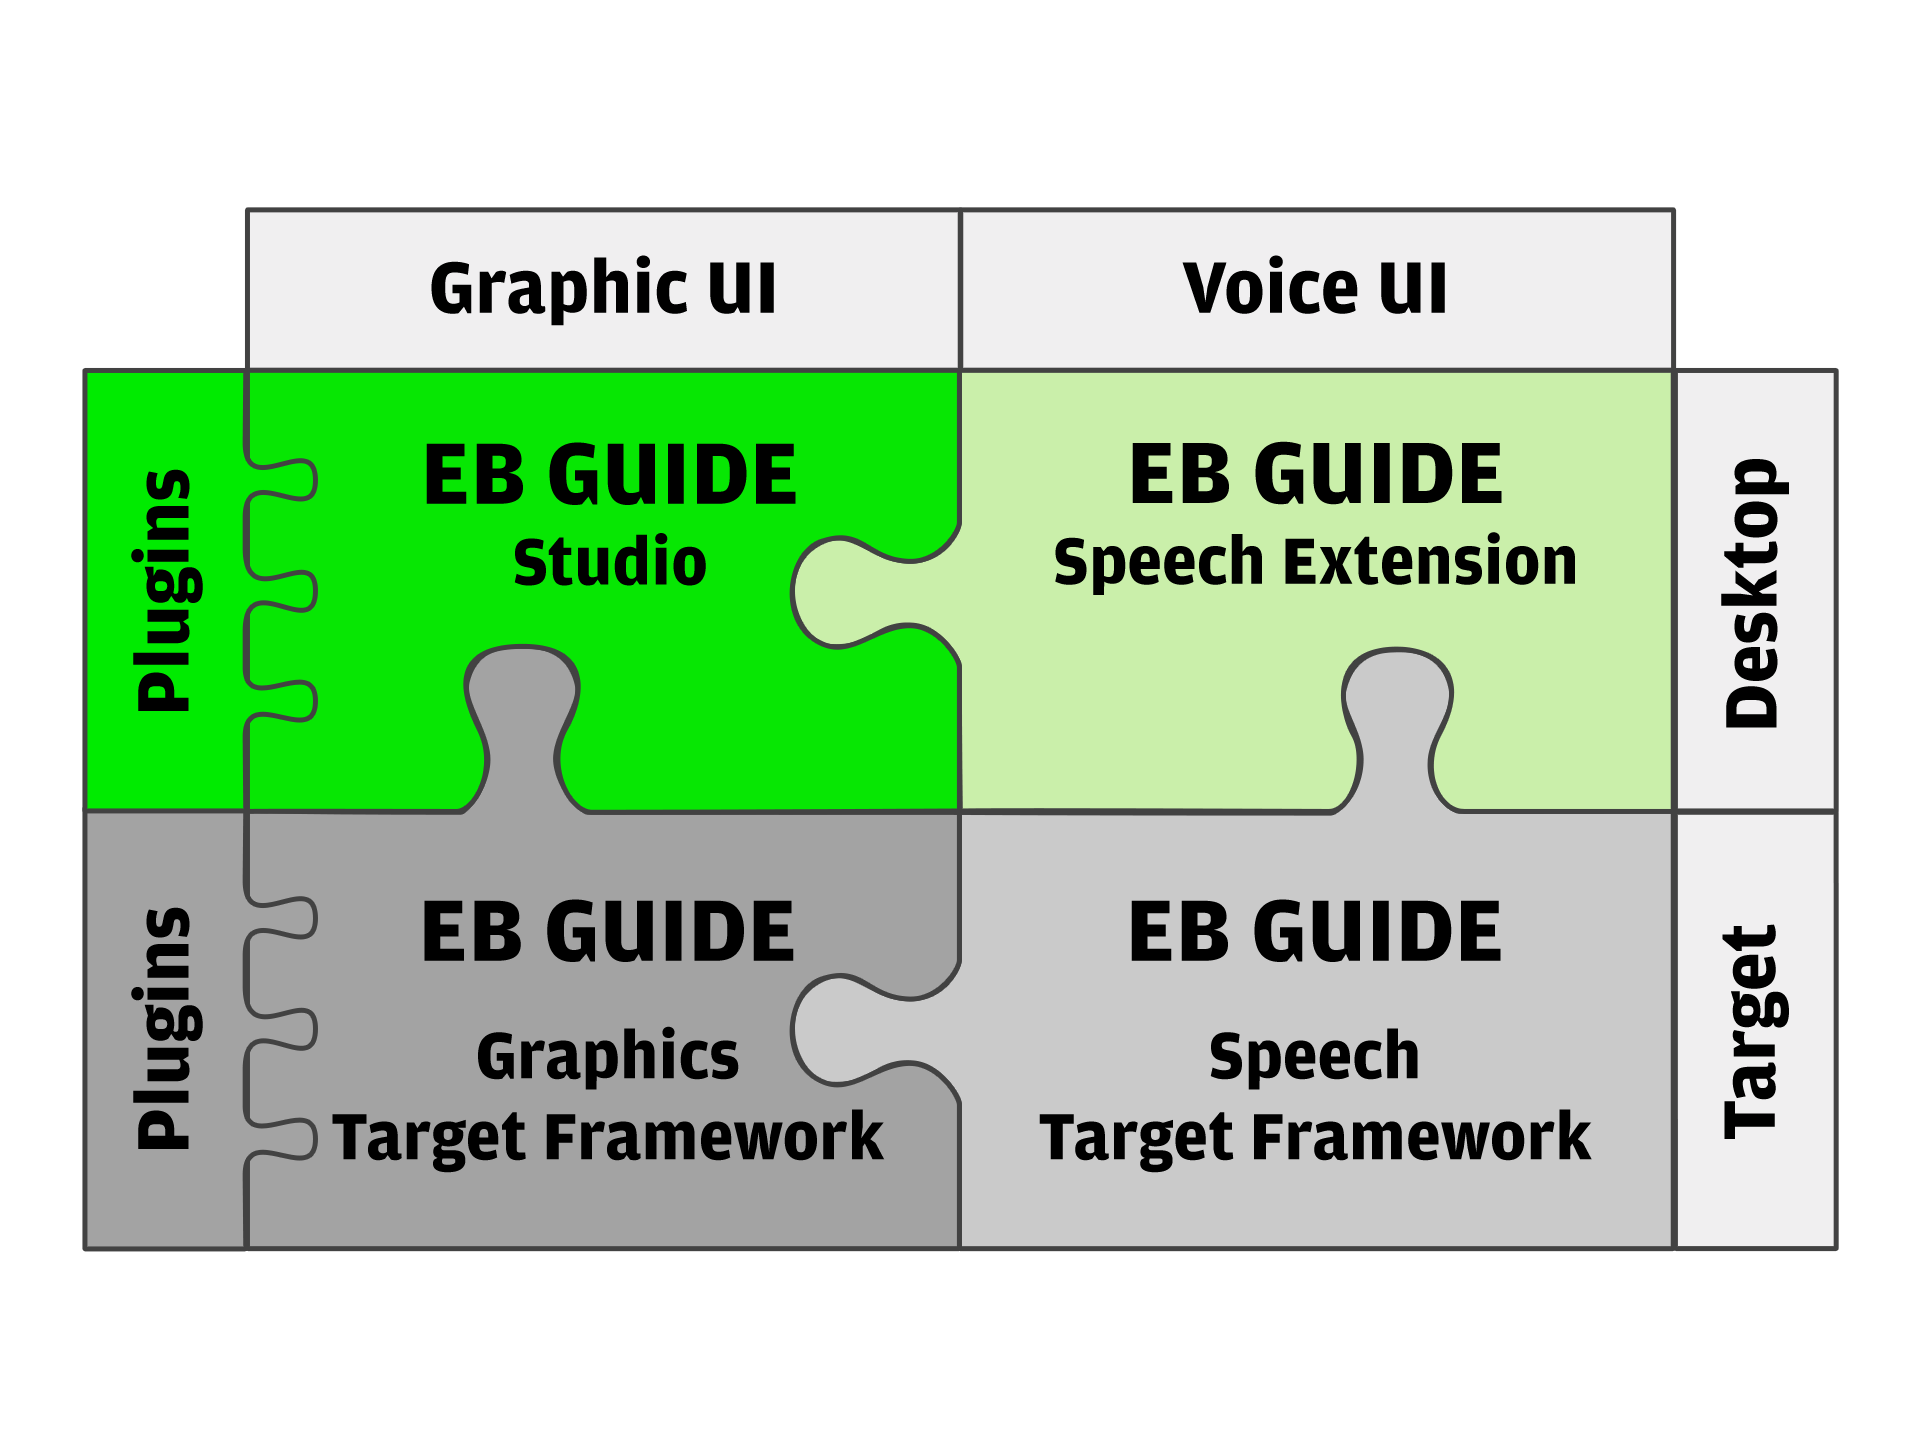
\includegraphics[scale=0.7]{figures/EB_GUIDE_Puzzle.png}
  \caption{Aufbau EB GUIDE}
  \label{fig:guide_puzzle}
\end{center}
\end{figure}

EB Guide Studio ist das Interface von EB Guide mit dem nach dem What-You-See-Is-What-You-Get (WYSIWYG) Prinzip User Interfaces modelliert werden. 
Durch das WYSIWYG Prinzip ist es während des Modellierens einer View bereits möglich das Endergebnis des Designs zu sehen.
Das Verhalten des Interfaces hingegen wird mithilfe einer Zustandsmaschine, der sogenannten Statemachine, modelliert die auf dem UML- Prinzip aufbaut.
Die Trennung der Logik und des Designs wird in EB GUIDE Studio grafisch durch zwei unterschiedliche Arbeitsoberflächen gestaltet in welchen den Modellierern jeweils die entsprechenden Tools und Elemente zur Verfügung stehen.

\begin{figure} [!h]
\begin{center}
  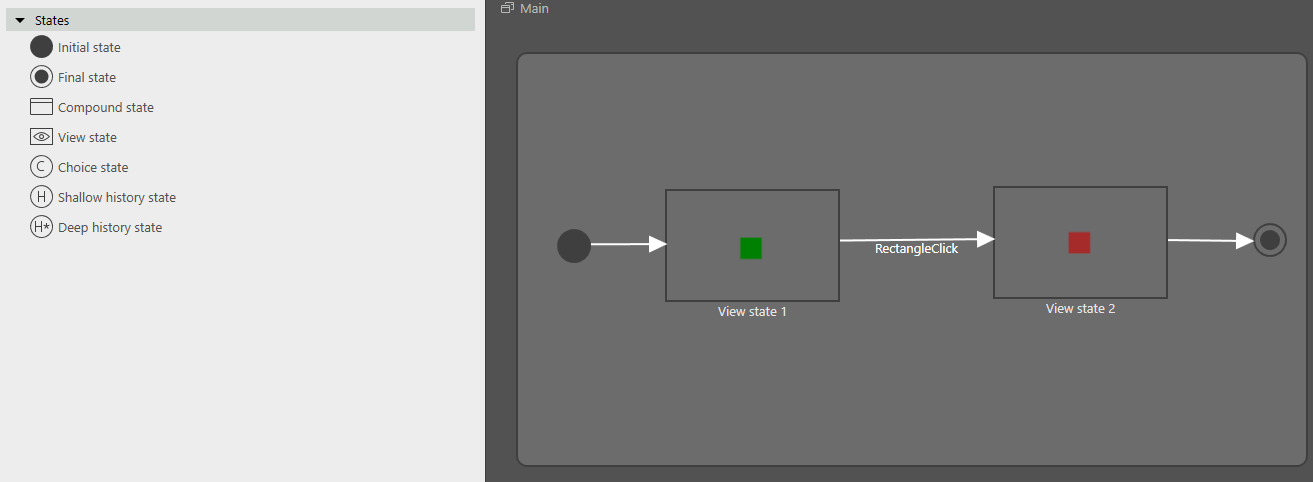
\includegraphics[scale=0.4]{figures/Guide_Statemachine.PNG}
  \caption{EB Guide Studio Statemachine}
  \label{fig:Guide_Statemachine}
\end{center}
\end{figure}

In \cref{fig:Guide_Statemachine} ist die Statemachine für ein simples Beispiel zu sehen.
Links neben der Arbeitsfläche befindet sich eine Toolbox mit deren Inhalt per Drag and Drop auf der Arbeitsfläche die benötigte Logik definiert wird.
Wie bei UML-Diagrammen gibt es einen Initial State der den Startpunkt angibt und einen Final State der die Statemachine beendet.
Die ebenfalls zu sehenden View States stehen für einen Screen im Endprodukt, dementsprechend wird in den View States auch das Aussehen der Interfaces definiert.
Die Verbindungen zwischen den States werden als Transitionen bezeichnet und mithilfe von Events ausgelöst.
Events stellen hierbei beliebige Ereignisse dar die durch Elemente in der View ausgelöst werden können.
Der Auslöser für das Event wird mithilfe einer eigens für EB Guide entwickelten Skriptsprache als Trigger für dieses gesetzt.
Die häufigsten Auslöser sind Benutzeraktionen mit Widgets, die in \cref{fig:Guide_View}zu sehen sind.
Widgets sind Elemente mit denen das Aussehen des Interfaces im sogenannten View Editor bestimmt wird und die sich in Basis- und 3D-Widgets einteilen lassen.
Alle Basiswidgets verfügen über Basiseigenschaften wie Höhe, Breite und Farbe sowie über spezifische Eigenschaften wie zum Beispiel "Touch-Released" bei einem Button.\cite{studio_guide}
Beipspielsweise wird das Event "RectangleClick", was sich in \cref{fig:Guide_Statemachine} an der Transition zwischen View State 1 und View State 2 befindet in diesem Beispiel durch das Klicken auf das grüne Rechteck in View State 1 ausgelöst.
Ist die Benutzeraktion abgeschlossen findet der Übergang von View State1 zu View State 2 statt und der Nutzer sieht nun anstatt dem grünen ein rotes Rechteck.
Damit diese Aktion erfolgreich ausgeführt wird muss das grüne Rechteck die Eigenschaft "Touch-Released"\ zugewiesen bekommen und über die EB Guide Skriptsprache mitgeteilt bekommen das Event RectangleClick zu feuern sobald das grüne Rechteck berührt wurde.
Da sich dieses Event in der Statemachine an der Transition zwischen den beiden States befindet wird nun durch einen Klick auf das grüne Rechteck ein Bildschirmwechsel zwischen den beiden View States ausgelöst.

\begin{figure}[!h]
\begin{center}
  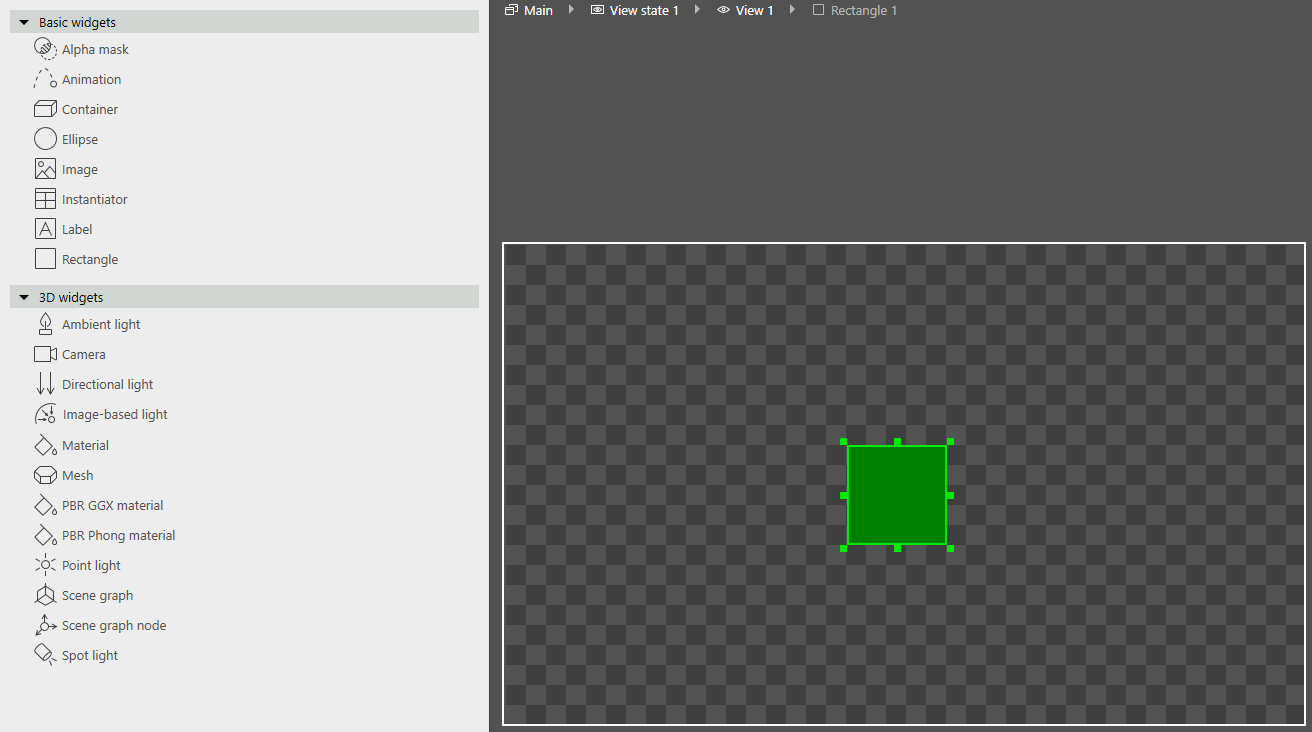
\includegraphics[scale=0.4]{figures/Guide_View.PNG}
  \caption{EB Guide VIEW}
  \label{fig:Guide_View}
\end{center}
\end{figure}


